\section{Introduction}
\section{Results}\label{sec:results_p2}

\subsection{Hysteresis curve}

Bijels have proposed applications as soft matter based material templates, drug delivery vectors and separations systems. 
The materials performance in each application is dependent upon the microstructure of the bijel template. Many of the 
applications listed above benefit from stimuli response, allowing for in-situ microstructure tuning to modify permeability 
of the material. We want to understand whether bijels provide access to reversible structural modifications which would 
allow stimuli responsive bijels to be used in in-situ applications.

We begin our investigation by characterizing the microstructure changes observed on bijels stabilized with prolate 
ellipsoids with a particle volume fraction of $\phi_p = 0.1$. We apply a constant magnetic field of $\bar{B}_z = 0.2$ 
onto bijels that were simulated with no magnetic field. Once the microstructure has reached its new state, we ramp up 
the magnetic field to $\bar{B}_z = 0.5$ and finally $\bar{B}_z = 1$. We then apply the opposite procedure to reduce 
the applied field strength, resulting in a magnetic field ramp of 
$\bar{B}_z: 0 \rightarrow 0.2 \rightarrow 0.5 \rightarrow 1 \rightarrow 0.5 \rightarrow 0.2 \rightarrow 0$.

We characterize the microstructure changes observed through calculating a characteristic length scale, 
called the average domain size. The average domain size is calculated using the first moment of the 3D 
averaged structure factor. Past work has shown that this method correctly reproduces the scaling expected 
in phase separating systems. The structure factor is calculated from the fourier transform of the fluctuations 
in the order parameter. \cite{kendon_inertial_2001}

We identified that this measure of the domain size tended to overestimate the domain size. However, past work has 
shown that the scaling behavior of the first moment derived domain size is consistent with phase separation expected 
for spinodal decomposition. Overestimation is caused by a low number of samples at small k values as the bin size is 
approximately equal to the k value. Furthermore, the structure factor and the length scale calculated in simulations
 with periodic domains are subject to finite size effects. Nevertherless, trends about the average domain size can be 
 determined from this measurement.

Before the structure factor was calculated, the location of the particles were filled with the average density of the 
surrounding lattice sites using Equation \ref{eq:fill_particles} to generate a smooth interface. The particles are 
iteratively filled from outside in until all lattice points corresponding to the particle are filled with the average 
density of the fluid surrounding the lattice point. Within the red and blue fluid densities, sites representing the 
particles are filled before the order parameter is calculated. By filling the particles, we are able to analyze the 
microstructure without the influence of the particles. We calculate the hysteresis curve by calculating the domain 
size at the final timestep of each magnetic field change. We then plot these domain sizes against the magnetic field 
applied to obtain them and split them in the descending and ascending magnetic field directions to demonstrate the 
differences observed. We plot these results in Figure \ref{fig:hysteresis_curve}

\begin{figure} 
    \centering 
    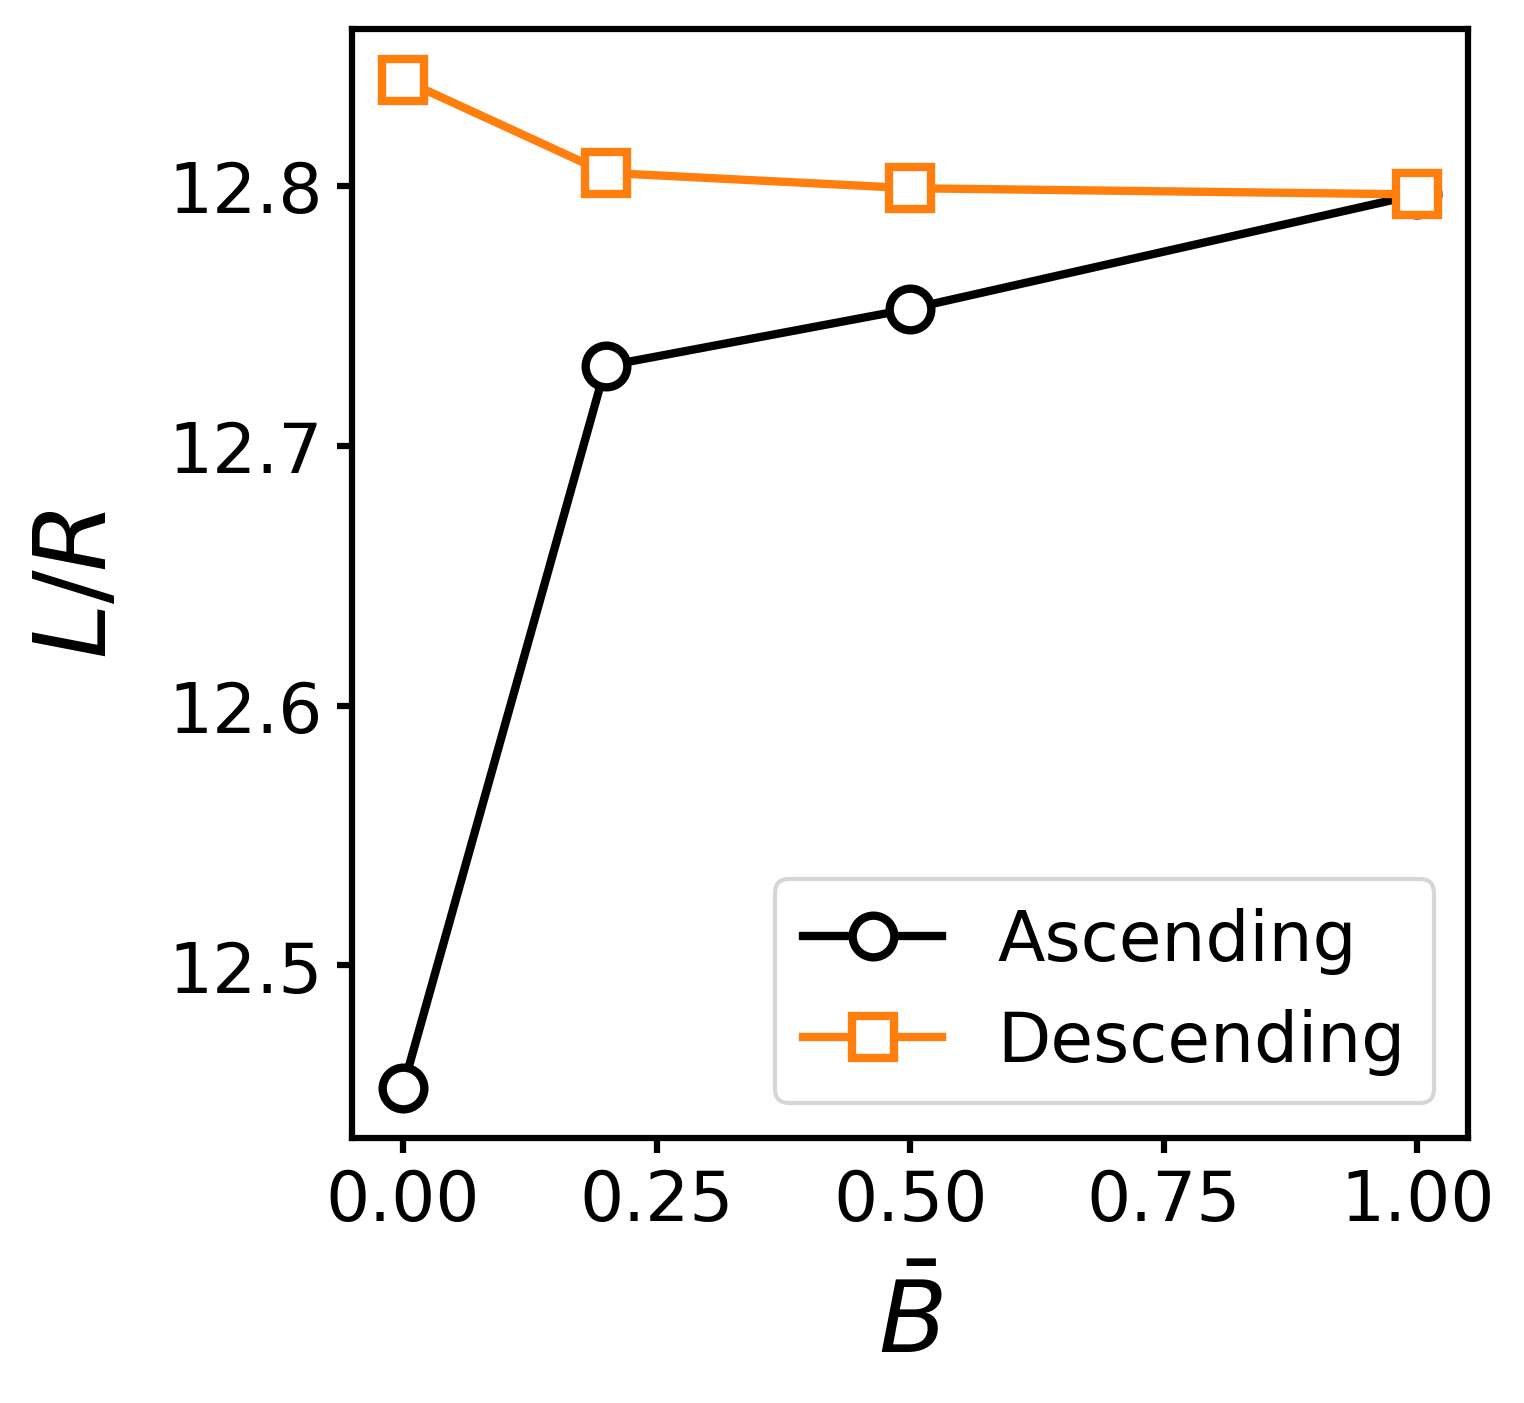
\includegraphics[scale=0.7]{../figures/results/paper2/hysteresis_curve.png} 
    \caption{Hysteresis curve of bijels stabilized with magnetically responsive ellipsoidal particles. The y-axis is the average length scale $\frac{L}{R}$ normalized with the radius of the particle, while the x-axis corresponds to the dimensionless magnetic field strength $\bar{B}$. We show that there is domain coarsening upon increase of the field strength, followed by jamming of the structure as the field strength is decreased indicating the path dependence of the bijel microstructure.} 
    \label{fig:hysteresis_curve} 
\end{figure}

Figure \ref{fig:hysteresis_curve} illustrates the hysteresis behavior of magnetically responsive bijels. 
We observe a hysteresis response of the bijel microstructure, characterized by a non-return of the microstructure 
to the original average domain size value when reducing the applied magnetic field strength. The increase in the 
average length scale when applying the magnetic field is due to domain coarsening caused by reorientation of particles 
to the magnetic field strength, reducing the interfacial coverage. When decreasing the magnetic field strength, 
we observe that the domain size does not return to the original value meaning that that the microstructure of the 
bijel is unaffected by the reduction in magnetic field. This suggests that the particles at the interface are in a 
kinetically trapped configuration.

\subsection{Applying a field}

We saw in Figure \ref{fig:hysteresis_curve} that there was hysteresis in the structural response of magnetic bijels 
to a constant magnetic field. The first facet to investigate would be why there is a large increase in the domain size 
between $\bar{B}_z: 0.0 \rightarrow 0.2$. In many of the proposed stimuli responsive applications for bijels, the 
timescales of response is important to characterize and would also provide a mechanistic understanding of the reasons 
why the microstructure changes. We probe these aspects of structural response of bijels in this section by assessing 
the response of bijels stabilized by particles with volume fraction of $\phi_p = 0.1$ simulated under no applied field 
to an applied field in the range $\bar{B} = 0, 0.2, 0.5, 1$. We begin our investigation by visualizing the structure 
before and after the application of magnetic fields. 

\begin{figure} 
    \centering 
    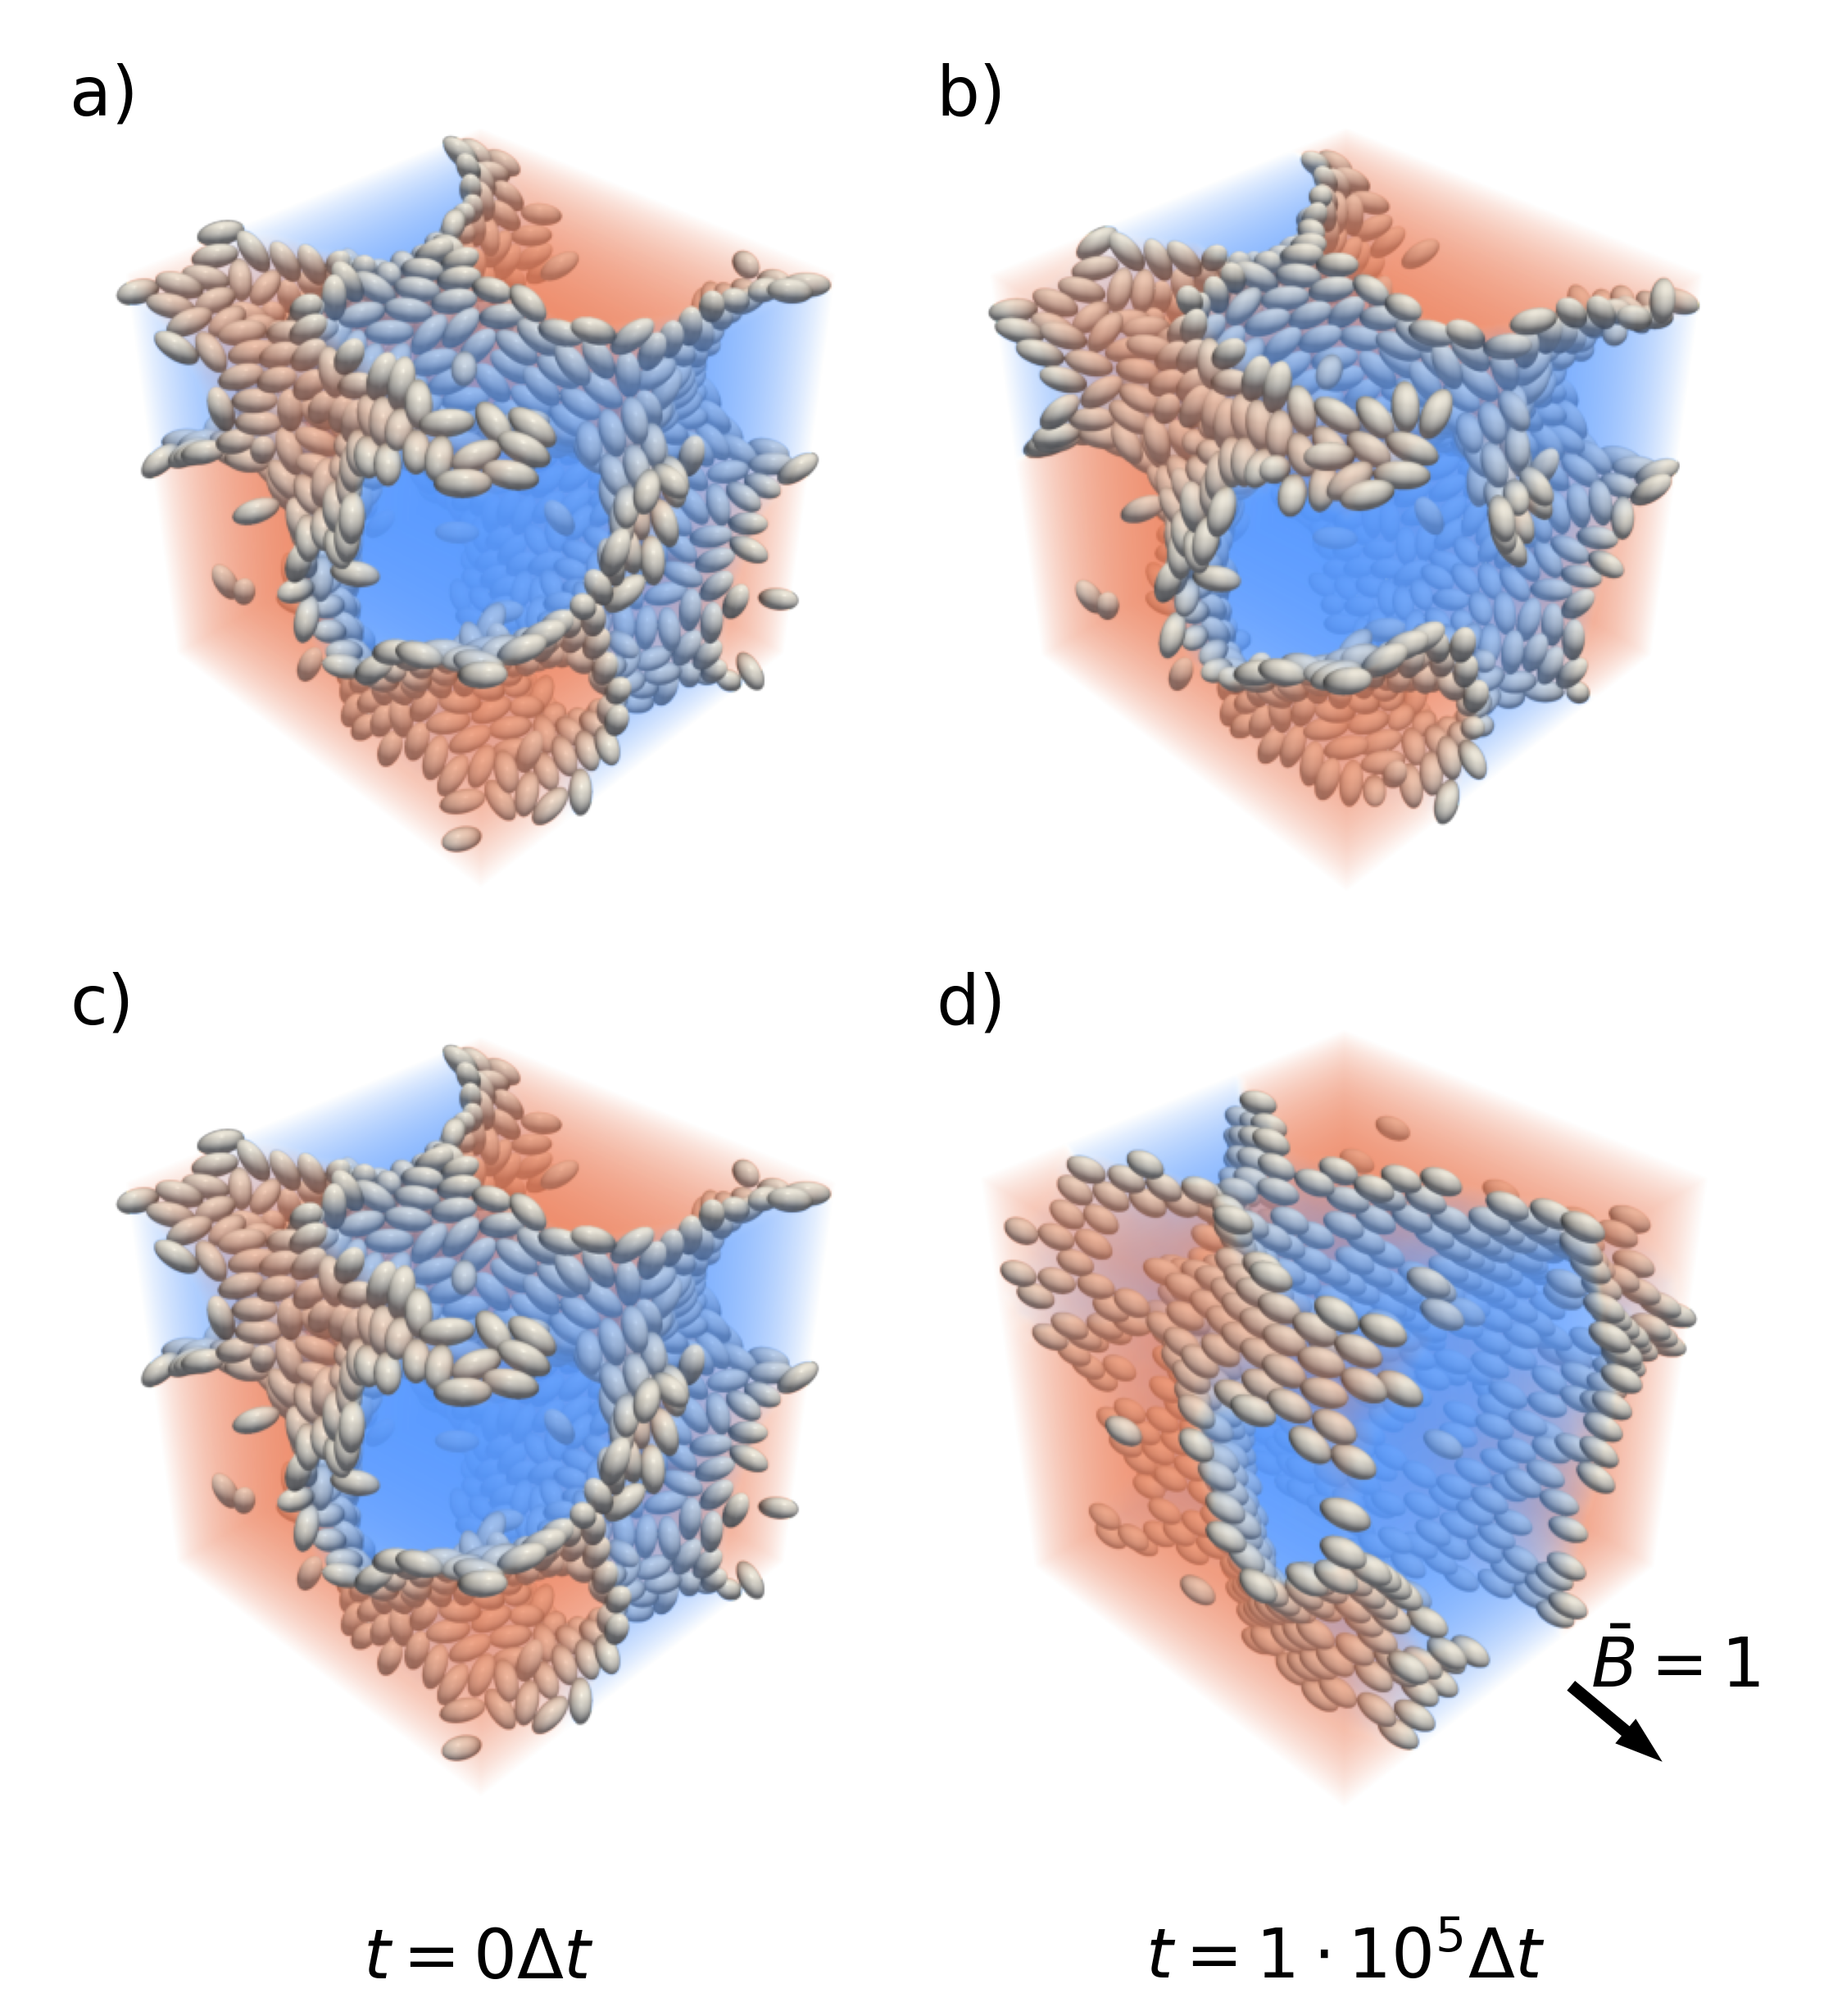
\includegraphics[scale=0.7]{../figures/results/paper2/microstructure_viz-field_on.png} 
    \caption{Visualizations of bijels simulated under no fields at $t = 0$ (left) and $t = 10^5$ (right). The top 
            column demonstrates the microstructure evolution if no field is used while the bottom column demonstrates 
            the microstructure evolution when the system is exposed to a field strength of $\bar{B} = 1$. Particle 
            reorientation to the direction of the field can be seen, resulting in microstructure changes driven 
            through domain coarsening until the particles jam.} 
    \label{fig:microstructure_viz-field_on} 
\end{figure}

In Figure \ref{fig:microstructure_viz-field_on} we show representative snapshots of the bijel at the initial and 
final timestep with $\bar{B}_z = 0$ and $\bar{B}_z = 1$. We show that upon application of the field, particles align 
to the direction of the field. As the particles orient to the field, they disrupt the packing of particles at the 
interface, causing domain coarsening as the particles rearrange into new positions. The particles then rejam in 
place once the interfacial area and particle cross sectional area match. Domain coarsening observed in the figure 
can be explained through the ordering of particles at the interface, causing a reduction in the available area that 
the particles have for stabilization. To correlate the microstructure evolution to the ordering of the particles, we calculate the 
nematic order parameter. \cite{cuesta_monte_1990} 

\begin{figure} 
    \centering 
    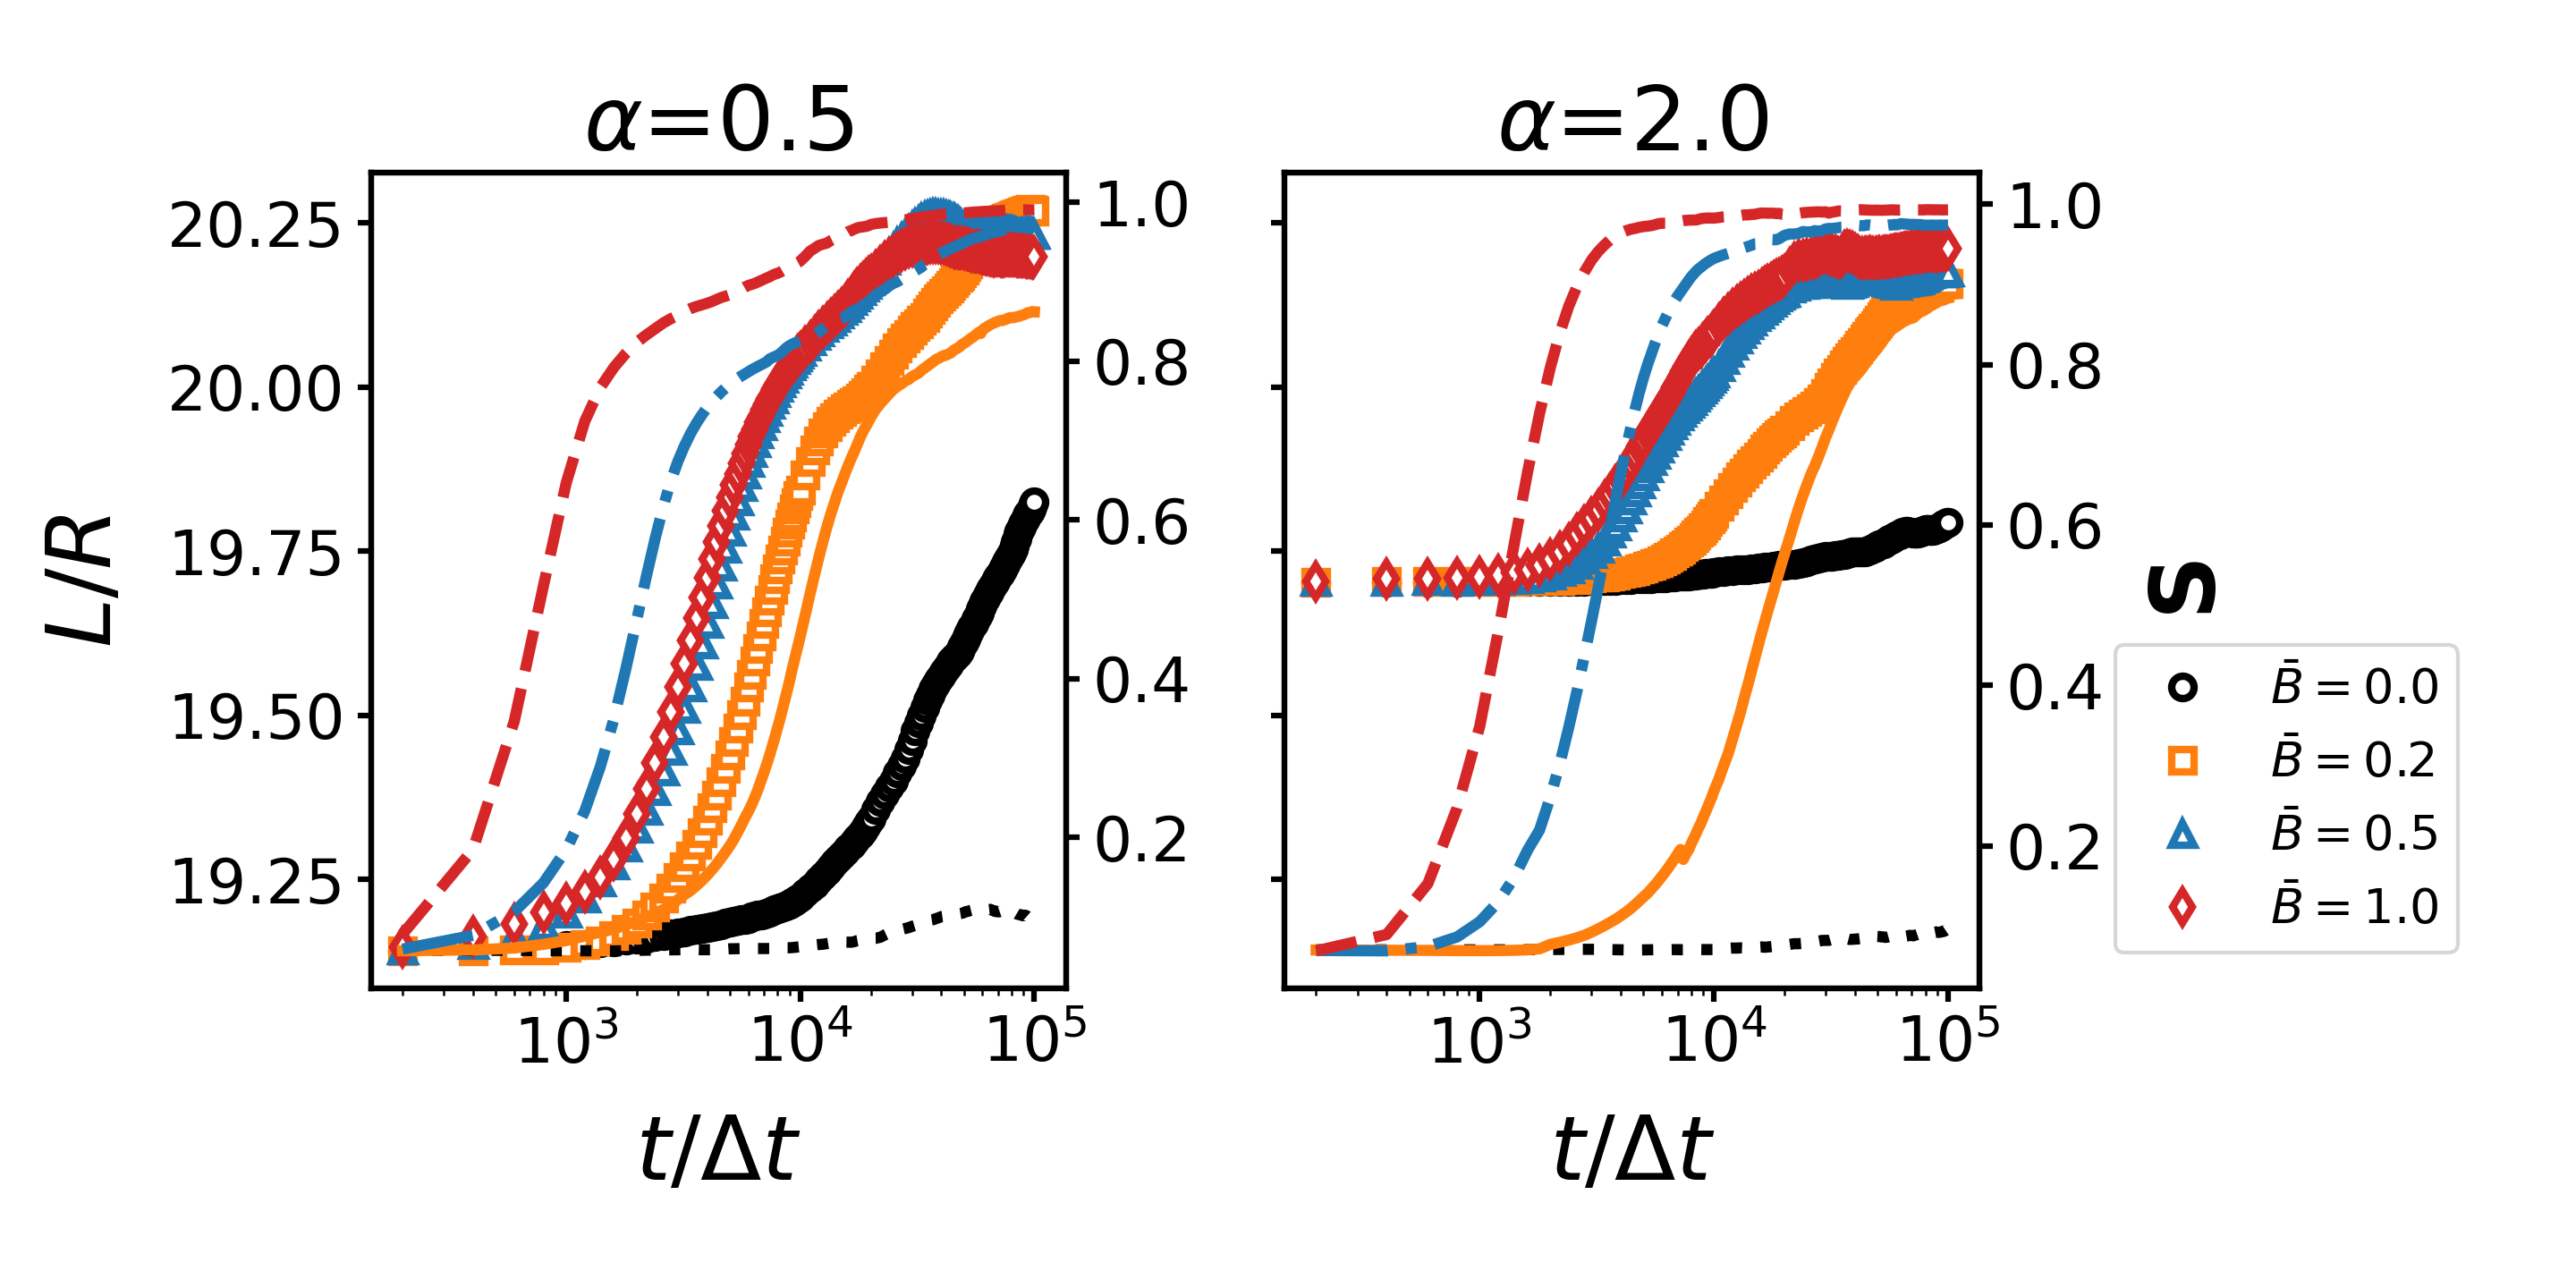
\includegraphics[scale=0.7]{../figures/results/paper2/domain_size-field_on.png} 
    \caption{Plotting the spherically averaged domain size normalized with $R_p$($L/R$) of the 
             particle at different magnetic field strengths, $\bar{B}$, and the nematic order parameter $S$ in lines.
             We quantify the domain size and ordering of the particles, and show that the change in both parameters
            are correlated with the strength of the applied magnetic field.} 
    \label{fig:domain_size-field_on} 
    \end{figure}

In Figure \ref{fig:domain_size-field_on}, we plot the average domain size change over time normalized by the particle 
radius parallel to the symmetry axis $R_p$. We see that there is a $\approx 2.4\%$ increase in the average domain size 
observed when switching on a magnetic field onto a bijel made with no field when comparing the final timestep of each 
simulation. We also observe that with no applied field, there is a small increase in the domain size. The 
microstructure change observed with no applied magnetic field is consistent with what Gunther et al. observed 
in their investigations on the timescales of bijels stabilized with ellipsoidal particles. \cite{gunther_timescales_2014} 
They concluded that domain size increases at long time scales seen in bijels stabilized with ellipsoidal particles 
occur due to steric force derived particle reorientation to a closer packed configuration, causing domain coarsening 
as the stabilized interface area reduces.

In Figure \ref{fig:domain_size-field_on}, we also plot the nematic order parameter of each respective bijel as 
lines demonstrating the change in this parameter over time. Firstly, we see the effect of particle reordering due 
to steric effects at $\bar{B}_z = 0$ from the slight increase $S$ over time. We also see that there is field 
strength dependence on the rate of ordering and final ordering of the particles to the field. A gap between the 
time evolution of the nematic order parameter and the domain size can be observed when $\bar{B}_z = 0.5, 1$, 
that is not present when $\bar{B}_z = 0.2$. It was hypothesized that the time taken for particle reorientation 
to the field would control the degree and rate of domain size change when the bijel begins with particles with 
random order. This result suggests that the dynamics of the system at higher magnetic field strengths are 
dependent upon other factors that vary upon application of the magnetic field.

We have also identified that bijels stabilized with anisotropic particles under magnetic fields form anisotropic 
structures. Past work has shown that the microstructure, specifically the length scale and tortuosity are critical to 
the performance of porous materials in applications such as battery electrodes and tissue engineering applications. 
\cite{zhang_promoting_2019, ebner_tortuosity_2014, hsieh_architected_2021} Characterization of the anisotropic 
microstructure would allow application specific microstructure design. To quantify the length scales in each cartesian 
direction, we also calculate the 2nd moment derived structure factor without radial averaging. \cite{jansen_bijels_2011} 
Once the structure factor is calculated as in Eq \ref{eq:structure_factor_calc}, the second moment of the structure factor 
in direction $\beta$ is calculated in each cartesian direction. We also calculate the tortuosity of the microstructures. In 
previous work, we identified that the length scale derived from the second moment of the structure factor is only useful 
for identifying length scale anisotropy. Therefore, we plot the directional second moment derived length scales and 
tortuosity in Figure \ref{fig:domain_size_aniso-field_on}.

\begin{figure} 
    \centering 
    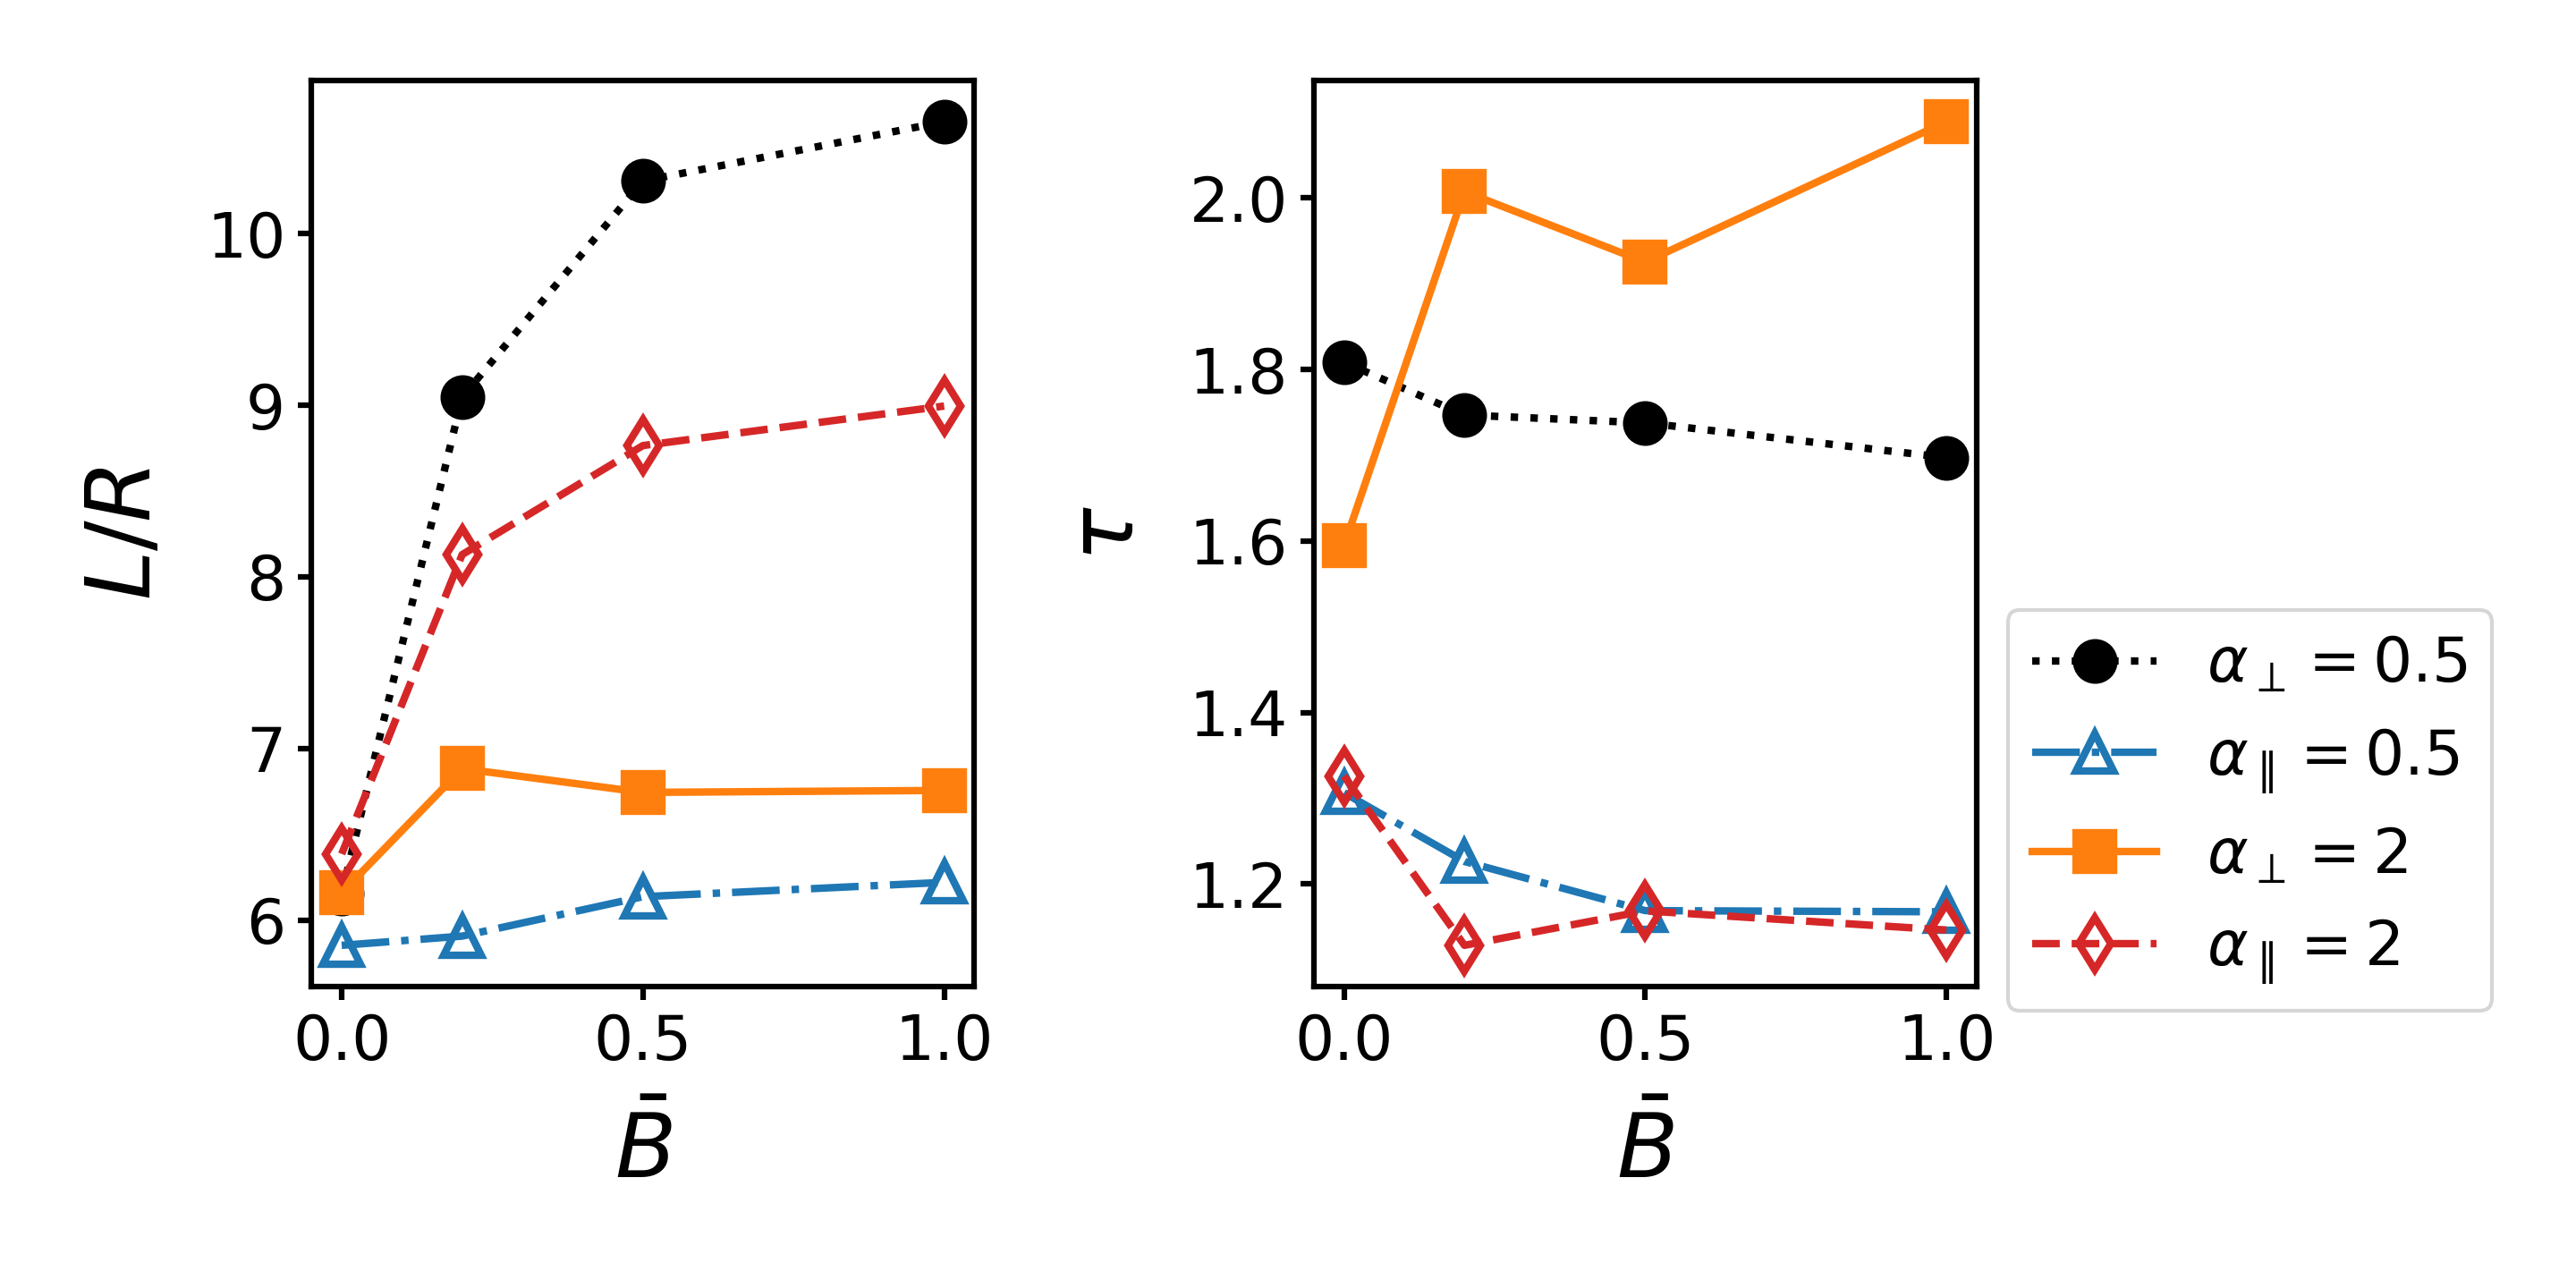
\includegraphics{../figures/results/paper2/domain_size_aniso-field_on.png} 
    \caption{Plotting the anisotropic domain size and tortuosities against the applied magnetic field strength on 
             the left and right respectively for bijels stabilized with magnetically responsive prolate ellipsoids. 
             We see that upon application of the field, the domain size parallel to the applied field direction, 
             $L_{\parallel}$ increases while the domain size perpendicular to the applied field, $L_{\perp}$ decreases.
             These results support the tortuosity data obtained which show that $\tau_{\parallel}$ decreases, 
             indicating a shorter path length, while $\tau_{\perp}$ increases, indicating a longer path length.} 
    \label{fig:domain_size_aniso-field_on} 
\end{figure}

From Figure \ref{fig:domain_size_aniso-field_on}, we see that domain size anisotropy is observed upon application of the field, with $L_{\perp}$ and $L_{\parallel}$ increasing and decreasing by 35 $\%$ and 13 $\%$ respectively. The qualitative changes match what has been observed in our past work when applying magnetic fields onto bijels during formation. \cite{karthikeyan_formation_2024} This can be explained through understanding the mechanisms of domain size change in both cases. During the formation of bijels, the particles are adsorbed onto the interface and oriented to the field when they jam, creating the anisotropic microstructure observed. In this case, we see that the particles reorient in response to the field, unjamming and rejamming once the domains have coarsened sufficiently that the interfacial area matches the area covered by the particle monolayer. The directionality of particles, causes domain ordering as the particles jam in their ordered states, causing domain size anisotropy in both cases.

In Figure \ref{fig:domain_size_aniso-field_on}, we demonstrate that the application of the magnetic field changes the 
domain size. The tortuosity of the bijel is initially around $\tau \approx 1.6$, consistent with simulations of the 
diffusive tortuosities of gyroid structures using Lattice Boltzmann simulations. \cite{luo_macroscopic_2020} 
Upon application of the field, $\tau_{\perp}$ slightly decreases while $\tau_{\parallel}$ increases. We have seen 
that an increasing domain size decreases the tortuosity in our past work. \cite{karthikeyan_formation_2024} This 
observation is in line with the domain size changes observed in Figure \ref{fig:domain_size_aniso-field_on}. The 
results show that the tortuosity of the bijel is noticeably affected by the application of magnetic fields. 
Earlier, we observed that the dynamics of structural response were not directly tied to the nematic order 
parameter upon application of stimuli. To understand this phemomena, we focus more on the dynamics of the 
particle monolayer. First, we visualize the particle monolayer of the bijels at the initial and final configuration 
before and after application of a magnetic field.

\begin{figure} 
    \centering 
    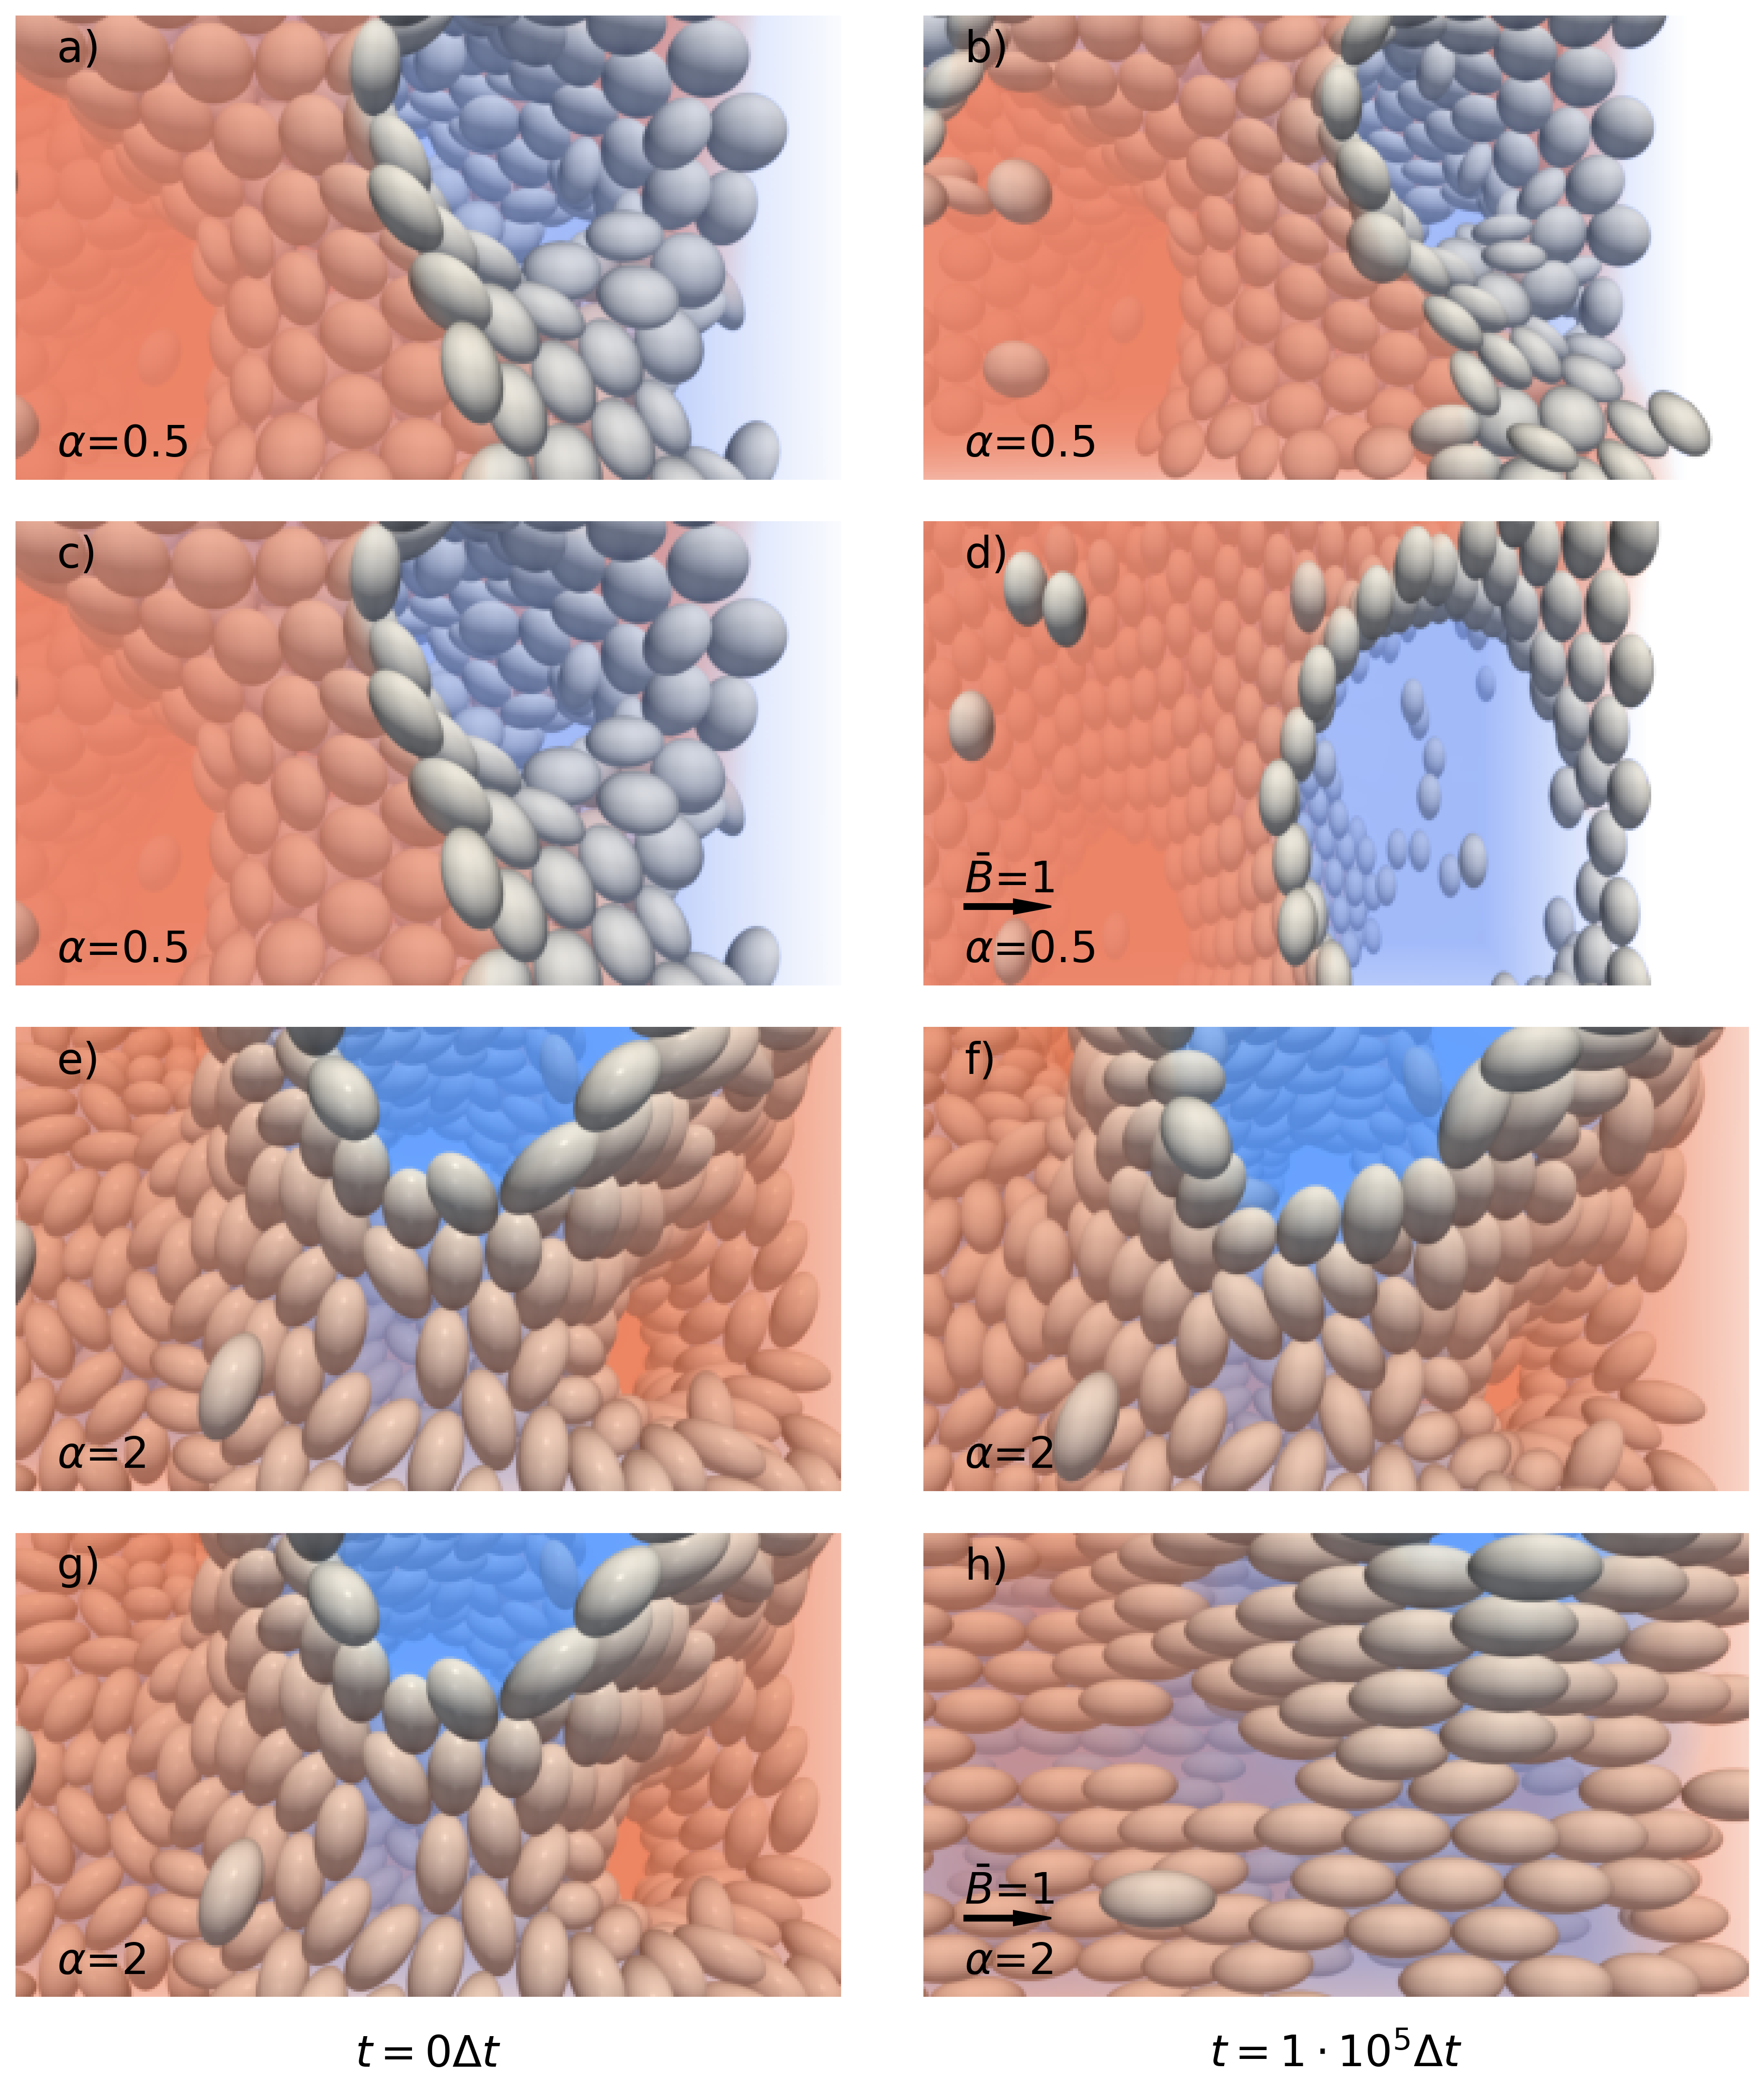
\includegraphics[scale=0.7]{../figures/results/paper2/particle_viz-field_on.png} 
    \caption{Visualizations of bijels simulated under no fields at $t = 0$ (left) and $t = 10^5$ (right). 
            The top column demonstrates the microstructure evolution if no field is used while the bottom column 
            demonstrates the microstructure evolution when the system is exposed to a field strength of $\bar{B}_z = 1$. 
            Particle reorientation to the direction of the field can be seen, resulting in coarsening of the domains.} 
    \label{fig:particle_viz-field_on} 
\end{figure}

In Figure \ref{fig:particle_viz-field_on}, we see the effect of the application of the magnetic field on the monolayer. 
The initial configuration of particles at the monolayer show that the orientations are random and that the particles 
tend to lie flat on the interface. However, upon application of the magnetic field the particles orient to the field 
direction. The effect that Gunther. et al. observed for bijels stabilized with anisotropic particles can also be 
observed in these snapshots as the particles can be observed to have more local order in the final state than in 
the initial state. 

Past work by Bresme and Faraudo and Davies investigating the reorientation of particles at interfaces under magnetic 
fields have shown that a critical magnetic field exists, above which the particle orients to the field and below 
which the particle orientation is a function of the capillary force and magnetic field derived force. 
\cite{davies_interface_2014, bresme_orientational_2007} Particle adsorption into the interface with microparticles have 
also been shown to be irreversible due to the high adsorption energy. Upon particle reorientation, the microstructure 
change can be driven solely through particle unjamming and re-jamming, or it can be driven through the particles dragging 
the interface during this process. The mechanism of unjamming and re-jamming can be investigated using the average 
interfacial angle, $\psi$.

Another factor affected by the application of the magnetic field is the Steinhardt 6 fold order parameter, $Q6$, 
which characterized the local particle ordering. \cite{steinhardt_bond-orientational_1983} It has been used to 
characterize crystallization, glass transitions and crystal structures for colloidal and molecular crystals. 
We utilize the average across all particles on the interface, $\langle Q6 \rangle$ and track this parameter 
as a function of time. Past work has identified that local crystallization of colloidal crystals takes place 
at $\langle Q6 \rangle = 0.38$, and that $\langle Q6 \rangle^{HCP} = 0.485$. 
\cite{steinhardt_bond-orientational_1983, toxvaerd_role_2020, mickel_shortcomings_2013}

From Figure \ref{fig:interface_angle-nint-field_on}, we see that the initial value of $\psi \approx 80 ^{\circ}$ 
indicating that at the start of the simulation, most of the particles lie flat on the interface. The variance from 
the expected $\psi = 90 ^{\circ}$ can be expected from the presence of the curved interface, meaning that not all 
particles will lie completely flat. This can also be seen in the microstructure visualizations in Figures 
\ref{fig:microstructure_viz-field_on} and \ref{fig:particle_viz-field_on}. Upon application of the field, 
$\psi$ decreases in all cases indicating that the particles are being oriented out of the interface. 
However, the energy of adsorption is sufficiently high that the interface moves with the particle as it 
reorients to the field. This is exhibited by the small change in $\psi$ and recovery to the initial value over time.

We also observe from plotting $\langle Q6 \rangle$ over time that the application of magnetic fields on bijels causes a 
local crystallization of the particle monolayer, as observed from the increase in $\langle Q6 \rangle > 0.38$ not 
observed when a magnetic field is not applied. We also observe that for $\bar{B} > 0.2$, $\langle Q6 \rangle$ will 
end up around $\langle Q6 \rangle = 0.45$ which indicates that they are close to being hexagonal close packed. 
This is related to the nematic ordering of the particles causing the local arrangement of particles to become 
more ordered. However, the arrangement of particles will not evolve at the same rate as the nematic order parameter 
as the local arrangement of particles will experience steric hindrance during rearrangement at the interface. 

Figure \ref{fig:domain_size-field_on}, we observed a gap between the growth of the nematic order parameter and an 
increase in the domain size. To probe why this occurs, we recast $\langle \psi \rangle$, $\langle Q_6 \rangle$ and 
$S$ in terms of the physical phenomena they represent. The nematic order parameter represents the ordering of 
particles to an average direction, which in the case of the application of a magnetic field, is the field direction. 
Therefore, a timescale reliant on the nematic order parameter would represent a timescale of response rate limited 
to the response to the magnetic field, which indicates a particle-field orientation dependence. We name this 
timescale $\tau_S$. When applying a field to a bijel system with a randomly oriented particle monolayer, the 
most significant transition point is the isotropic to nematic transition or when $S \geq 0.3$. We define $\tau_S$ 
for this section of the analysis by identifying when $S \geq 0.3$.

We can also do the same for $\langle \psi \rangle$ and $\langle Q_6 \rangle$. A timescale derived from 
$\langle \psi \rangle$ named $\tau_{\langle \psi \rangle}$ represents the capillary timescale between the 
interface and the particle which is also affected by interparticle interactions. Given the shape of the plot,
we assign the $\tau_{\langle \psi \rangle}$ to be the time when the first minimum of $\langle \psi \rangle$ is 
observed. A timescale derived from $\langle Q_6 \rangle$, named $\tau_{\langle Q_6 \rangle}$ is also calculated. 
This represents the point when local crystallization of the particle monolayer occurs, calculated when 
$\langle Q_6 \rangle \geq 0.38$. We omit $\bar{B} = 0$ as previous results have identified the domain size 
changes observed there. We then plot the average domain size $L$ against time rescaled with these three 
timescales in Figure \ref{fig:domain_size-field_on-scaled}.

\begin{figure} 
    \centering 
    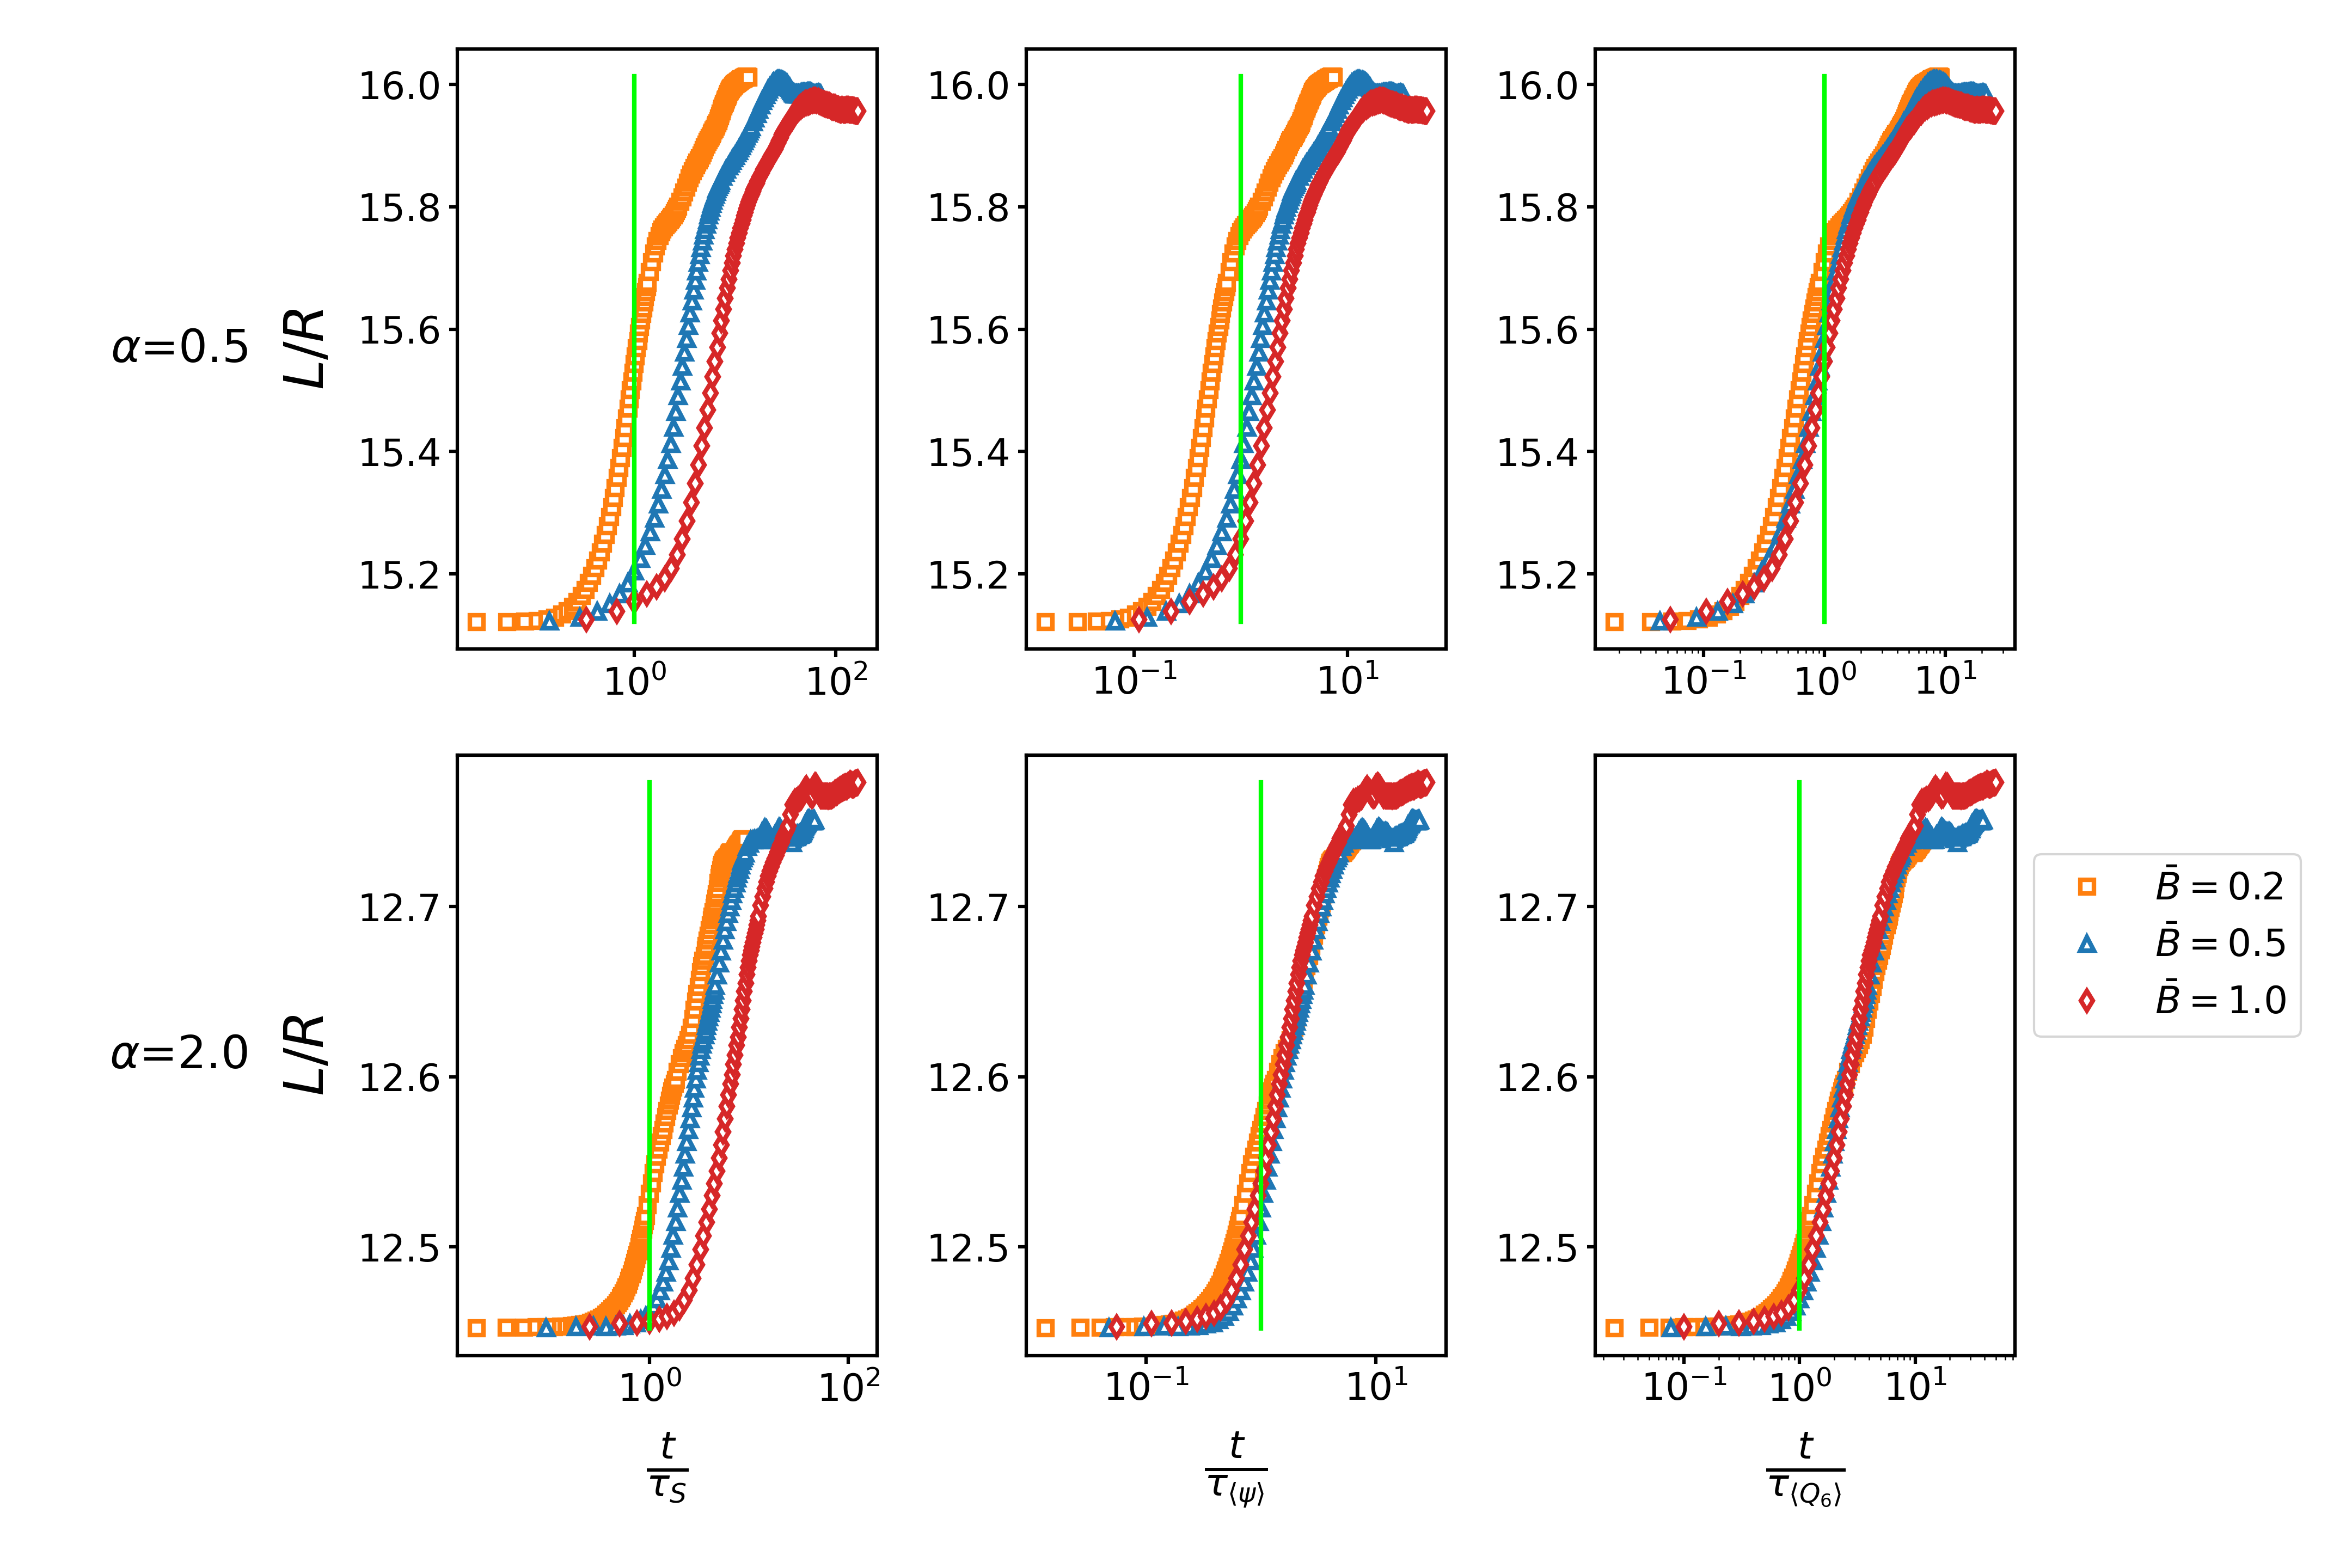
\includegraphics{../figures/results/paper2/domain_size-field_on-scaled.png} 
    \caption{Plots of domain size with different timescales. The figure on the left rescales time with the nematic to 
            isotropic transition time while the figure on the right rescales time with the time taken till the 1st minimum in 
            the interface angle is reached. We show that the controlling timescale when applying a magnetic field onto bijels 
            with disordered particles is the latter timescale, indicating that the dominating effect is steric hindrance as the 
            interface is dragged along with the particles upon reorientation.} 
    \label{fig:domain_size-field_on-scaled} 
\end{figure}

In Figure \ref{fig:domain_size-field_on-scaled}, the left plot plots the average domain size against time rescaled 
using $\tau_S$. We see that the domain sizes do not collapse onto a single line, which is expected if we want to 
explain the dynamics using the nematic order parameter. This confirms the observation made above that the dynamics 
do not only depend on the reorientation of particles to the field. The middle plot demonstrates the average domain 
size against time rescaled using $\tau_{\langle \psi \rangle}$. We see that there is good agreement between all 
simulations, although the point when $\frac{t}{\tau_{\langle \psi \rangle}} = 1$ lies when the domain size transition 
has started. The right plot demonstrates the domain size change after rescaling time with $\tau_{\langle Q_6 \rangle}$ 
where we see good collapse between all plots while the domain size transition also begins at 
$\frac{t}{\tau_{\langle Q_6 \rangle}} = 1$. The latter point demonstrates that the dynamics for the 
structural response of randomly oriented particles are controlled by the local particle rearrangement at the 
interface rather than the orientation of the particle to the magnetic field.

From the evidence in Figure \ref{fig:domain_size-field_on-scaled}, two types of interfacial behaviors are characterized 
in addition to that identified by Gunther et al. \cite{gunther_timescales_2014} The first type is what is observed for 
$\bar{B} = 0.2$, where the interfacial coverage and average orientation of the particle to the field and to the 
interface change in lock step. This causes the interface to reorient at the same rate as the particles reorienting 
to the magnetic field. The second is observed for $\bar{B} = 0.5, 1$, where there is a time lag between particle 
ordering, and the intiation of domain coarsening. In the latter scenario, at early times the particles are jolted 
out of position before the large adsorption energy of the particles into the interface causes the interface to move 
to the particle position, causing domain coarsening as the interfacial area reduces. 

\subsection{Increasing the applied field strength}

\subsection{Reducing the applied field strength}